\documentclass[]{article}
\usepackage{graphicx}
\usepackage[T1]{fontenc}
\usepackage{array}
\usepackage{tabu}
\graphicspath{{/home/shenoy/Documents/Nikhil/research/RADICAL-research/testing/summary/}}

\begin{document}
\title{Performance Summary of Ensemble-MD Patterns}
\author{Nikhil Shenoy}
\date{\today}
\maketitle

\abstract{Modern software, no matter its application, always incorporates performance as a design factor. Without efficient algorithms and implementations, the software becomes less attractive to the user because it does not accomplish the user's tasks in a timely fashion. Such factors are seriously considered when designing software for scientific computing, as many simulations in areas such as molecular dynamics require efficient tools to process the ever-increasing amount of data. In this article, we discuss the EnsembleMD-Toolkit and benchmark the efficiency of three standard Patterns using a sample workload. We assume that the reader has a basic familiarity with the Toolkit, and we will define only parameters relevant to the performed experiments.}

\section{Experiments}
	\subsection{General Parameters}
		These performance experiments were designed to analyze the Pipeline, Simulation Analysis, and Replica Exchange Patterns. Using these Patterns, we execute a two-stage workload; the first stage consists of creating a 10Mb file of random characters, and the second stage performs a character count on this file. In Table 1, we have included the commands used to execute each stage as well as the average execution time from the Bash Shell. We also use the environment parameters specified in Table 2.

		\begin{table}[h!]
			\centering
			\begin{tabu}{|c|c|c|}
				\hline
				Kernel & Bash Command & Avg. Execution (seconds) \\
				\hline
				misc.mkfile & base64 /dev/urandom | & .008 \\ 
							& head -c 100 > test.txt \\
				\hline
				misc.ccount & grep -o . test.txt |  & .004\\ 
							& sort | uniq > out.txt   \\
				\hline
			\end{tabu}
			\caption{Kernels, their commands, and their expected execution times.}
		\end{table}

		\begin{table}[h!]
			\centering
			\begin{tabular}{|c|c|}
					\hline
					Parameter & Value \\
					\hline
					\hline
					EnsembleMD-Toolkit version & 0.3.14-27-g65bc062 \\
					\hline
					EnsembleMD Branch & devel \\
					\hline
					RADICAL-Pilot version & 0.40.1 \\
					\hline
					Target Machine & XSEDE Stampede \\
					\hline
			\end{tabular}
			\caption{Environment Parameters.}
		\end{table}

	\subsection{Types of Scaling}
		For these experiments, we measured performance as a function of the number of cores allocated to a script as well as the number of instances of the Pattern being executed. We initially implemented weak scaling, in which the number of cores scales at the same rate as the number of instances, with the goal of observing a relatively constant execution time. The intuition behind this is that the core to instance ratio stays the same, which implies that the work per core/instance combination is the same. We also perform strong scaling, in which we hold the number of instances constant while we scale the number of cores. In this case, we expect that the Pattern will make use of the additional cores to finish the task more quickly. The scale that we use for these experiments is [1,16,32,64,128].

		In each script, we measured the time taken to complete various stages of execution. These will be elaborated upon in the subsection for each pattern.

	\subsection{Pipeline}
		For the Pipeline pattern, we measured the parameter of each defined in Table 3.

		\begin{table}[h!]
		\centering
			\begin{tabular}{|c|p{10cm}|}
				\hline
				Parameter & Definition  \\
				\hline
				EnMD Core Overhead & (alloc\_stop-alloc\_start) +  (dealloc\_stop-dealloc\_start) \\
				\hline
				EnMD Pattern Overhead & ((step\_1\_wait-step\_1\_start) + (step\_1\_stop-step\_1\_res)) + \\ 
									  &	(step\_2\_wait-step\_2\_start) + (step\_2\_stop-step\_2\_res)) \\
				\hline
				RP Overhead & ((step\_1\_wait-step\_1\_res) - step\_1\_data\_movement - step\_1\_execution\_time) + \\
							&	((step\_2\_wait-step\_2\_res) - step\_2\_data\_movement - step\_2\_execution\_time) \\
				\hline
				Step 1 Execution Time & PendingAgentOutputStaging - Executing \\
				\hline
				Step 2 Execution Time & PendingAgentOutputStaging - Executing \\
				\hline
				Data Movement Time & ((Step\_1\_Done - Step\_1\_PendingAgentOutputStaging) + \\ 
								   &	(Step\_1\_Allocating - Step\_1\_StagingInput)) + \\
								   &	((Step\_2\_Done - Step\_2\_PendingAgentOutputStaging) + \\
								   &	(Step\_2\_Allocating - Step\_2\_StagingInput)) \\
				\hline
			\end{tabular}
			\caption{Pipeline Definitions}
		\end{table}

		\begin{figure}[h!]
			\centering
			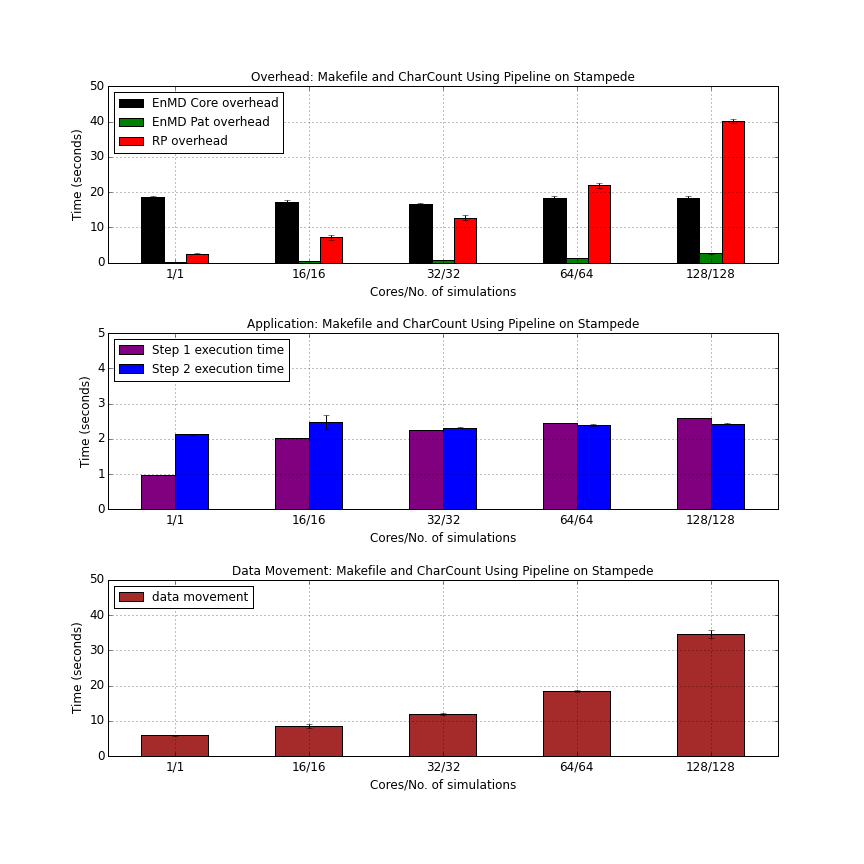
\includegraphics[scale=.30]{iteration_3/pipeline_weak_scaling.png}
			\caption{Weak Scaling with the Pipeline Pattern}
			\label{fig:pipeline_weak_scaling}
		\end{figure}

		Figure 1 shows the scaling behavior of each of the parameters. In the first graph, we observe that the EnsembleMD Core overhead stays relatively constant at about 18 seconds throughout the scaling. We also see that the EnsembleMD Pattern Overhead is at most 3 seconds, which is a fraction of the Core overhead. Finally, we see that the RADICAL-Pilot overhead increases rapidly as the scale increases. Ratios between RP overheads from a configuration to the previous configuration yield a value of about 1.8, which implies that the overhead is growing linearly.
		In the second graph of Figure 1, we see that the execution times for both Step 1 and Step 2, which were the Makefile and Character Count respectively, stay very much constant throughout the scaling, except for the anomaly of Step 1 in the first configuration. This is to be expected, as the settings in the configuration should have no effect on how long it takes to run the underlying Bash commands. However, the times shown are much larger than those observed when the commands are executed directly from a Bash prompt. It is possible that the extra time is due to overhead from a combination of EnsembleMD and RADICAL-Pilot, but we have not dissected this additional component.
		Finally, the data movement shows a steady increase in duration. The ratios from one configuration to the previous configuration fluctuate from 1.6 to 1.9, but generally imply a linear increase in time. 

		\begin{figure}[h!]
			\centering
			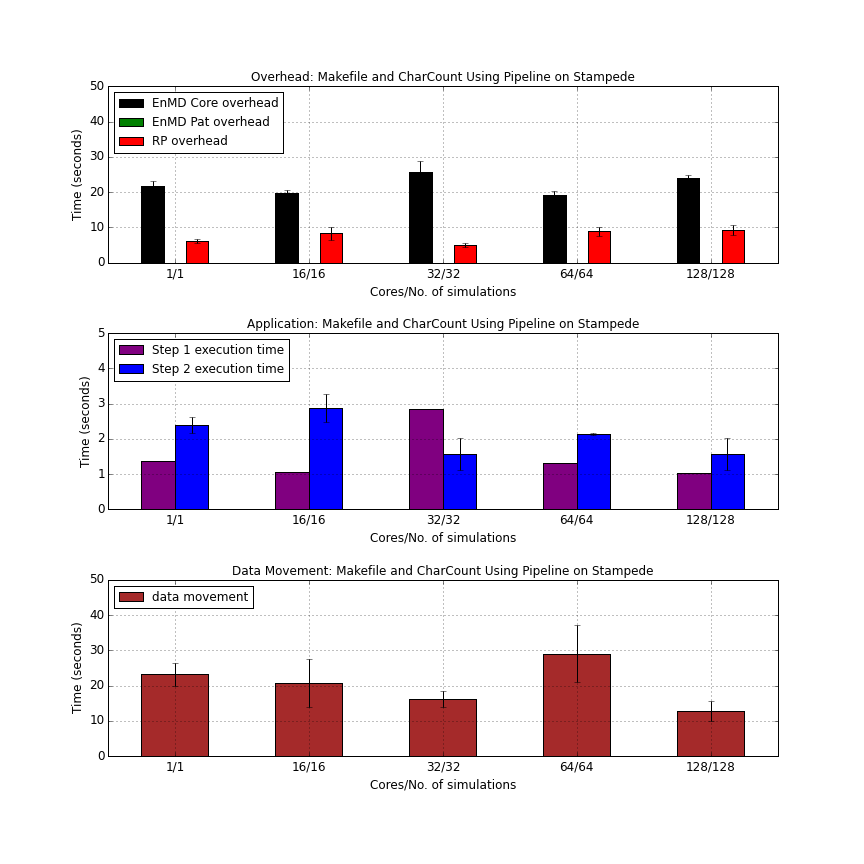
\includegraphics[scale=.30]{iteration_3/pipeline_strong_scaling.png}
			\caption{Strong Scaling with the Pipeline Pattern}
			\label{fig:pipeline_strong_scaling}
		\end{figure}

		Figure 2 displays the strong scaling results from the Pipeline. Looking at the EnsembleMD Core Overhead, we find that it averages to around 22 seconds. On the other hand, the Pattern Overhead was so small that they did not register on the scale of the Core Overhead. Finally, the RP overhead remains approximately constant at around 8 seconds. 
		The execution times for Steps 1 and 2 show a much different trend than they did in the weak scaling experiments. In general, Step 1 showed execution times that were closer to the actual execution time, but were still three orders of magnitude greater. Step 2 fluctuated much more than it did during the weak scaling experiments.
		Data movement shows a general decline in duration, aside from the anomaly with 64 cores. This may be due to the increased number of cores available for the movement.

	\subsection{Simulation Analysis}

		For Simulation Analysis, we considered the definitions in Table 4.

		\begin{table}[h!]
			\centering
			\begin{tabular}{|c|p{10cm}|}
				\hline
				Parameter & Definition  \\
				\hline
				EnMD Core Overhead & (alloc\_stop-alloc\_start) +  (dealloc\_stop-dealloc\_start) \\
				\hline
				EnMD Pattern Overhead & ((sim\_wait-sim\_start) + (sim\_stop-sim\_res)) + \\ 
									  &	((ana\_wait-ana\_start) + (ana\_stop-ana\_res)) \\
				\hline
				RP Overhead & ((sim\_wait-sim\_res) - sim\_data\_movement - sim\_execution\_time) + \\
							&	((ana\_wait-ana\_res) - ana\_data\_movement - ana\_execution\_time) \\
				\hline
				Simulation Execution Time & PendingAgentOutputStaging - Executing \\
				\hline
				Analysis Execution Time & PendingAgentOutputStaging - Executing \\
				\hline
				Data Movement Time & ((Step\_1\_Done - Step\_1\_PendingAgentOutputStaging) + \\ 
								   &	(Step\_1\_Allocating - Step\_1\_StagingInput)) + \\
								   &	((Step\_2\_Done - Step\_2\_PendingAgentOutputStaging) + \\
								   &	(Step\_2\_Allocating - Step\_2\_StagingInput)) \\
				\hline
			\end{tabular}
			\caption{Simulation Analysis Definitions}
		\end{table}

		\begin{figure}[h!]
			\centering
			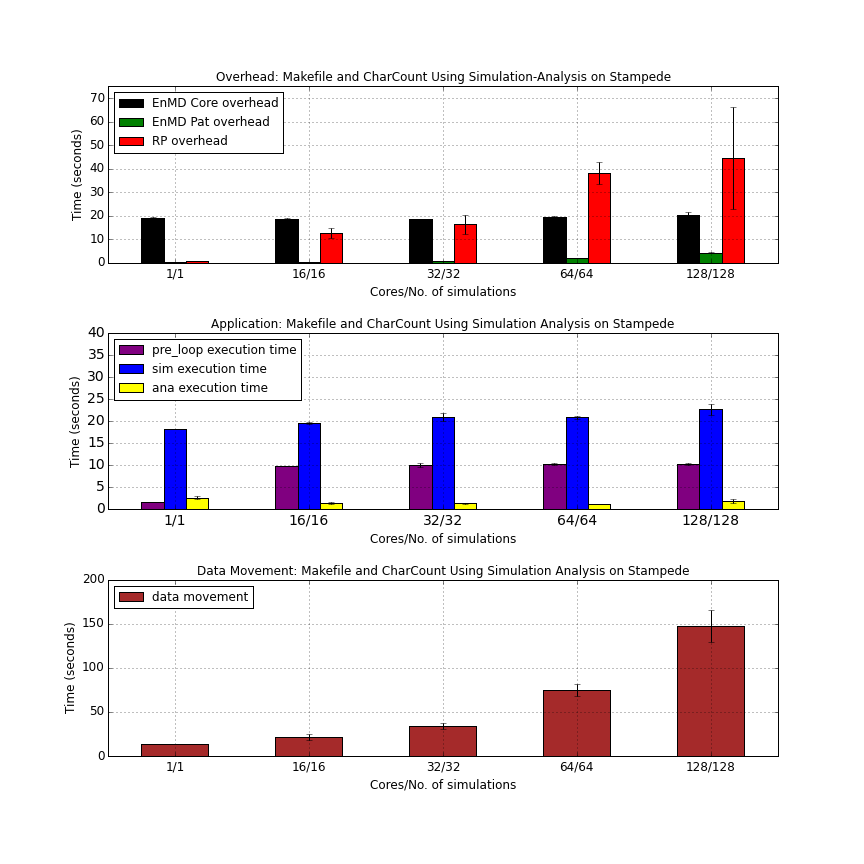
\includegraphics[scale=.30]{iteration_3/sa_weak_scaling.png}
			\caption{Weak Scaling with the Simulation Analysis Pattern}
			\label{fig:sa_weak_scaling}
		\end{figure}

		In Figure 3, we see scaling behavior similar to what we saw in the original pipeline weak scaling experiment. The EnsembleMD Core Overhead is essentially constant, the Pattern Overhead is small in comparison and is capped at around 5 seconds, and the RP overhead does show an increase across the combinations. However, the RADICAL-Pilot overhead does not show a distinct linear progression in the same fashion as the Pipeline Weak Scaling plot did. 
		The second plot shows the phases of execution of the experiment. The pre-loop phase contained no logic, so the inference is that the times shown are the overhead introduced to make the call to the pre-loop. The Simulation execution time, which contained the Makefile Kernel, was constant throughout the scaling, but took longer on average than it did for the Pipeline. The Character Count, encapsulated by the Analysis stage, was truer to the values recorded in the Pipeline Weak Scaling plot.
		The Data movement plot shows a similar increase in the time needed to download the output data, but the trend does not seem to be linear. 

		\begin{figure}[h!]
			\centering
			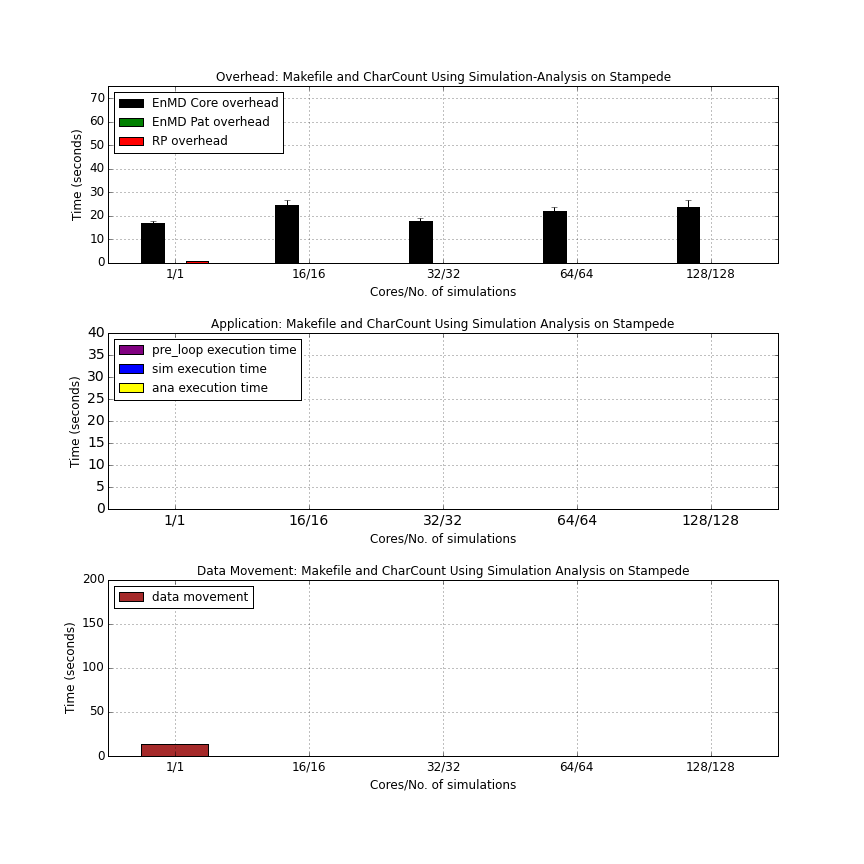
\includegraphics[scale=.30]{iteration_3/sa_strong_scaling.png}
			\caption{Strong Scaling with the Simulation Analysis Pattern}
			\label{fig:sa_strong_scaling}
		\end{figure}
		
		Finally, we examine the behaviors of each measurement during the Strong Scaling experiments with Simulation Analysis. EnsembleMD Core Overhead wavers around 20 seconds, whereas the RADICAL-Pilot Overhead has a large amount of variation in its time. While not pictured on the graph, the EnsembleMD Pattern Overhead does exist. The durations for those measurements were on the order of thousandths of a second, and thus would not be visible on the same graph.
		In the Simulation phase, we find that the execution time has been reduced dramatically, and that a representative value for it could be 13ms. The Analysis phase also varies slightly, but can be approximated at 7ms.
		The Data Movement durations are troubling, seeing as there is not a clear pattern to how the different values were obtained. The scaling does not seem to have had a visible effect on the duration of this phase.


\section{Future Work}
	Performance testing is an ongoing body of work in any scientific experiment. The results presented here can be extended into many different directions, and we propose some here. First, one could examine the relationship between the time taken to process varying sizes of data and the number of cores given to process that data. Such information would be useful in gauging EnsembleMD's capability to handle large and small amounts of data. The same experiments could be run on all the high performance machines supported by the Toolkit, with the expectation that the user gets similar performance no matter which machine he uses. The number of cores used to perform the scaling can also be increased; these experiments only went up to 128 cores, when it is becoming increasingly prevalent to have machines with up to 1024 availble cores. Extending these experiments to that augmented scale would help the EnsembleMD team adapt the Toolkit towards the increasingly common configurations.
\end{document}